\section{Gateway: Design \& Implementation}

\label{sec:gateway}
Having described our cryptographic building blocks, we can now discuss how they are used for encryption at the gateway.

\begin{figure}[t]
  \centering
  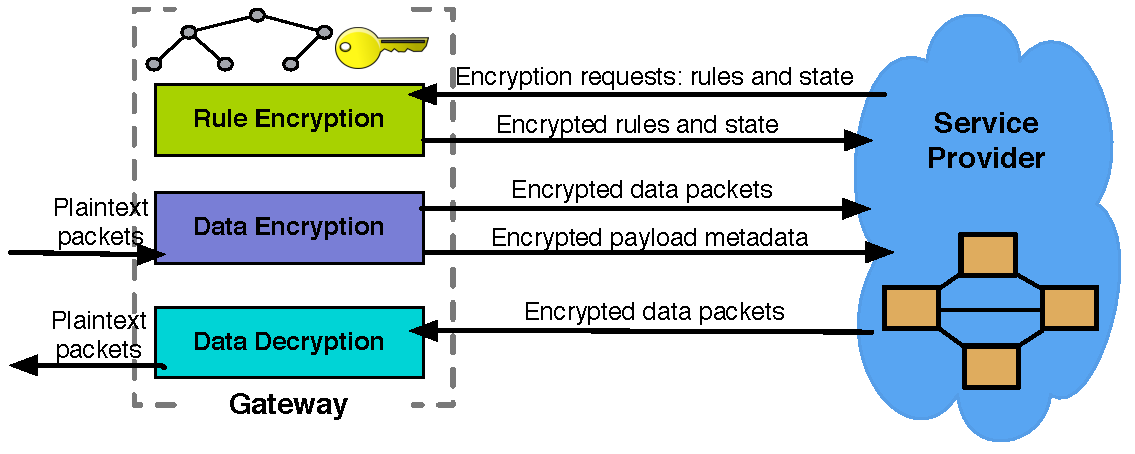
\includegraphics[width=3.25in]{fig/gateway2cloud}
  \caption[]{\label{fig:gatewaymeta} Communication between the cloud and gateway services: rule encryption, data encryption, and data decryption. \justine{Need to be consistent: is this a metadata channel or an extension channel}}
\end{figure}


\eat{
\begin{figure}[t]
  \centering
  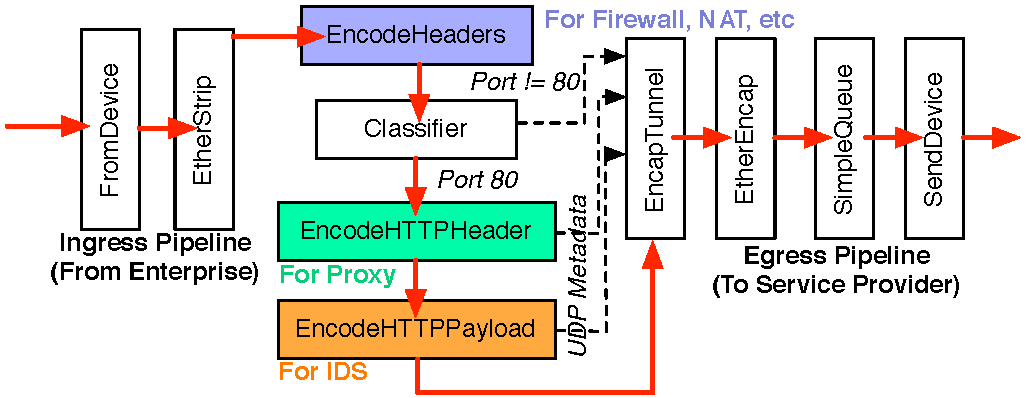
\includegraphics[width=3.25in]{fig/gatewaydiag}
  \caption[]{\label{fig:gateway} Data encryption (enterprise to cloud) click module.}
\end{figure}
}

The gateway serves two purposes. First, it redirects traffic to/from the cloud for middlebox processing. Second, it provides the cloud with encryptions of IDS/FW rulesets and updates to the RangeMatch tree.
Every gateway is configured statically to tunnel traffic to a fixed IP address at a single service provider point of presence.
A gateway can be logically thought of as three services: the rule encryption service, the pipeline from the enterprise to the cloud (Data encryption), and the pipeline from the cloud to the enterprise (Data decryption). 
All three services share access to the RangeMatch tree and the private key $k$.
Figure~\ref{fig:gatewaymeta} illustrates  these three services and the data they send to and from the cloud provider.

We design the gateway with two design principles in mind: 

\noindent{\bf Format-compatibility}: in converting plaintext traffic to encrypted traffic, the encrypted data should be structured in such a way that the traffic {\it appears as normal IPv6 traffic} to middleboxes performing the processing. This allows us to leave many middleboxes completely unmodified in how they perform per-packet operations, ensuring compatibility with optimizations including those in hardware (and hence good performance at the cloud). 

\noindent{\bf Scalability and Low Complexity}: the gateway should perform only inexpensive per-packet operations and should be parallelizable. The gateway should not require configuration other than to generate a key and establish a session with the cloud provider. If the gateway were as expensive and complex as the middleboxes themselves, the client would have no cost or management benefits from outsourcing. 

We now discuss how the gateway performs encryption and decryption (\S\ref{sec:dataenc}) and how rules are encrypted (\S\ref{sec:rulenc}) with these design goals in mind.

\subsection{Data Encryption and Decryption}
\label{sec:dataenc}

As shown in Table~\ref{tbl:mbreqs}, we categorize middleboxes as Header middleboxes, which operate only on IP and transport headers; HTTP middleboxes, which operate on HTTP headers and may operate on IP and transport headers; and DPI middleboxes, which operate on arbitrary fields in a connection bytestream. 
We discuss how each category of data is encrypted/decrypted in order to meet middlebox requirements as follows.

\subsubsection{IP and Transport Headers}
IP and Transport Headers are encrypted field by field (\eg{}, a source address in an input packet results in an encrypted source address field in the output packet) with RangeMatch.
We use RangeMatch for these fields because many middleboxes perform analysis over prefixes and ranges of values -- e.g., a firewall may block all connections from a restricted IP prefix.

\noindent{\bf Decryption.} RangeMatch is not reversible. To enable packet decryption, We store the AES encrypted values for the header fields in the IP options header. When the gateway receives a packet to decrypt, it decrypts the values from the options header restores them to the IP or transport header.

\noindent{\bf Format-compatibility.} 
Our modifications to the IP and transport headers place the encrypted range match data back in to the same fields as the unencrypted data was originally stored; because comparisons between rules and encrypted data rely on $\leq$ $\geq$, just as unencrypted data, this means that operations performing comparisons on IP and transport headers {\it remain entirely unchanged at the middlebox.}
This ensures backwards-compatibility with existing software {\it and hardware} dataplane operations.
Because per-packet operations are tightly optimized in production middleboxes, this compatibility ensures good performance at the cloud despite our changes.

An additional challenge for format compatibility is where to place the decryptable AES data; one option would be to define our own packet format, but this could potentially lead to incompatibilities with existing middlebox software. By placing it in the IPv6 options header, middleboxes can be configured to ignore this data using standard configuration.\footnote{It is a common misconception that middleboxes are incompatible with IP options. Commercial middleboxes are usually aware of IP options but many administrators {\it configure} the devices to filter or drop packets with certain kinds of options enabled.}


\subsubsection{Payload Data} 
The connection bytestream is encrypted with KeywordMatch using a searchable encryption approach.
This allows \sys to support DPI middleboxes, such as intrusion detection or exfiltration prevention.
These devices must detect whether or not there exists an exact match for an encrypted rule string {\it anywhere} in the connection bytestream.
Because this encrypted payload data is over the {\it bytestream}, we need to generate encrypted values which span `between' packet payloads. 
Searchable Encryption schemes, which we use for encrypted DPI, require that traffic be {\it tokenized} and that a set of fixed length substrings of traffic be encrypted along a sliding window -- e.g., the word malicious might be tokenized into {'malici', 'alicio', 'liciou', 'icious'}.
If the term 'malicious' is divided across two packets, we may not be able to tokenize it properly unless we reconstruct the TCP bytestream at the gateway. Hence, if DPI is enabled at the cloud, we do exactly this.

The gateway transmits the encrypted bytestream over an `extension', secondary channel that only those middleboxes which perform DPI operations inspect. 
Other middleboxes ignore this extra data.



\noindent{\bf Decryption.} The payload data is encrypted with AES and placed back into the packet payload -- like RangeMatch, KeywordMatch is not reversible and we require this data for decryption at the gateway.
Because the extension channel is not necessary for decryption, it is not transmitted back to the gateway.

\noindent{\bf Format-compatibility.} To middleboxes which only inspect/modify packet headers, encrypting payloads has no impact. Once again we are still faced with the challenge of where to place the extra data in the form of the KeywordMatch values. By placing this data in the extension channel, the extra traffic can be routed past and ignored by middleboxes which do not need to operate over this data, hence it will not interfere with normal processing. 

DPI middleboxes which do inspect payloads must be modified to inspect the extension channel alongside the primary channel, as described in~\cite{blindbox}; DPI devices are typically implemented in software rather than hardware and and these modifications are both straightforward and introduce limited overhead (as we will see in \S\ref{sec:eval}). 

\subsubsection{HTTP Headers} 

HTTP Headers are a special case of payload data.
Middleboxes such as proxies, L7 load balancers, and parental filters do not read arbitrary values from packet payloads: the only values they read are the HTTP headers.
We treat these values specially compared to other payload data; we encrypt the HTTP URI using unsalted AES (which is deterministic) and store them in IP options header of the packet containing the request.

This optimization is useful for two reasons. 
First, when DPI is not enabled, we can extract and store the HTTP headers statelessly; so long as HTTP pipelining is disabled and packet MTUs are standard-sized (>1KB), the required fields will always appear contiguously within a single packet.
Hence, if DPI is disabled we can avoid reconstructing the TCP bytestream at the middlebox.
Second, when DPI is enabled, the gateway scans through every byte of data in the connection already;  extracting these headers allows the middlebox to avoid re-doing work which has already been done at the gateway.

\noindent{\bf Decryption.} The packet is decrypted as normal using the data stored in the payload; options are removed.

\noindent{\bf Format-compatibility.}
Once again, by placing the encrypted value in an IP options header, we can avoid conflicts that arise from defining our own protocol.
We do need to rewrite HTTP parsing devices but, like DPI devices, they are implemented in software and our modifications introduce no overhead (as discussed in \S\ref{sec:eval}).


\subsection{Rule Encryption}
\label{sec:rulenc}

We now discuss how encrypted rules are generated from plaintext rules at the gateway and how they are updated while the service is running.

\noindent\textbf{Rule generation.} Rules for firewalls and DPI services come from a variety of sources and can have different policies regarding who is or isn't allowed to know the rules. 
For example, exfiltration detection rules may include keywords for company products or unreleased projects which the client may wish to keep secret from the cloud provider. 
On the other hand, many DPI rules are proprietary features of DPI vendors, who may allow the provider to learn the rules, but not the client.
\sys supports three different models for KeywordMatch rules which allow clients and providers to share rules as they are comfortable: (a) the client knows the rules, and the provider does not; (b) the provider knows the rule, and the client does not; or (c) both parties know the rules.
RangeMatch rules only supports (a) and (c) -- the gateway who maintains the rule tree {\it must} know the rules to perform encryption properly.

If the client is permitted to know the rules, they encrypt them -- either generating a KeywordMatch, AES, or RangeMatch rule -- and send them to the cloud provider. If the cloud provider is permitted to know the rules as well, the client will send these annotated with the plaintext for each encryption; if the cloud provider is not allowed, the client sends only the encrypted rules in random order.

If the client is not permitted to know the rules, we must somehow allow the cloud provider to learn the encryption of each rule with the client's key. This is achieved using a classical combination of Yao's garbled circuits~\cite{Yao86} with oblivious transfer~\cite{Naor-Pinkas}, as originally applied by BlindBox~\cite{blindbox}.
As in BlindBox, this exchange only succeeds if the rules are signed by a trusted third party (such as McAffee, Symantec, or EmergingThreats) -- the cloud provider should not be able to generate their own rules without such a signature as it would allow the cloud provider to read arbitrary data from the clients' traffic.
Unlike BlindBox, this rule exchange occurs exactly once -- when the gateway initializes the rule. 
After this setup, all connections from the enterprise are encrypted with the same key at the gateway.
This is important because for a typical industry ruleset, a garbled circuit + oblivious transfer exchange takes 97 seconds~\cite{blindbox}; with BlindBox this exchange must be performed for every connection and thus is prohibitive for practicality.
For \sys, on the otherhand, this amounts to a relatively cheap one-time setup cost.

\textbf{Rule Updates.}
The gateway also handles updates to rules, which we discussed in \S\ref{sec:updates}.

\subsection{Implementation}
\label{sec:gwimpl}
We built our gateway using Click over DPDK on an off-the-shelf 16-core server with 2.6GHz Xeon E5-2650 cores and 128GB RAM; the network hardware is a single 10GbE Intel 82599 compatible network card. Our gateway datapath implementation has 3 major components: Header Rewrite, Stream Reconstruction, and Packet Cache. We primarily introduce the dataflow from the client to the gateway below:

\noindent\textbf{Header Rewrite.} At this stage, the gateway rewrites the header fields in the packets using the RangeMatch scheme using in algorithm in Section \ref{sec:dataenc}. It consists of multiple Click elements: ProtocolTranslator46 that translates an IPv4 packet to an IPv6 packet, AppendIP6Option that populates DET-encrypted header fields into the IPv6 options, HeaderEncrypt that performs the encryption, and SetTCPChecksum that sets the checksum.

\noindent\textbf{Stream Reconstruction.} This component acts as a TCP transparent proxy by terminating incoming TCP connections from clients. It encrypts the reconstructed bytestreams using the stream cipher, and relays them in new connections. Note that the IP options are preserved during this phase. It also pushes bytestreams into the secondary channel, where middleboxes can perform DPI operations. Meanwhile, it extracts HTTP headers from the stream and puts the deterministically encrypted HTTP header fields into the IP options.

\noindent\textbf{Packet Cache.} To optimize the bandwidth usage, the gateway temporarily caches the packets destined to the service provider indexed by their hashes for a short time. If the middleboxes on the cloud do not change the packet content, instead of sending the whole packet back, the service provider sends a control packet containing the hash of the original packet. The gateway then retrieves the local packet by looking up the hash in the cache.

The dataflow from the service provider back to the gateway is relatively simple. The Packet Cache restores the packets, the Stream Reconstruction component decrypts the streams into plaintext, then the Header Rewrite component decrypts the header fields and performs 6to4 translation (if the client uses IPv4).

Having discussed the design and implementation of the gateway, we now revisit a few of its system properties before moving on to the design and implementation of the middleboxes in \S\ref{sec:mbimpl}.

\noindent\textbf{Scalability.}
Encryption and decryption are entirely parallel: they require no synchronization or communication between threads. We show in \S\ref{sec:eval} that we achieve almost linear improvements from adding additional processing cores.
However, per-packet operations rely only on relatively inexpensive techniques; the most expensive operation performed is AES encryption with is supported in hardware through the AES-NI instruction~\cite{aes-ni}. 
Consequently, the gateway can support 10Gbps of traffic with only 8 cores enabled.

\noindent\textbf{Complexity.}
An administrator only supplies the gateway with the IP address of the cloud and the secret key $k$.
The administrator places the gateway at the border of their enterprise network to the Internet.
The administrator supplies any rules/policies to the cloud provider and the gateway is then configured by the cloud provider.

\noindent\textbf{Fault Tolerance.}
When DPI is disabled, the gateway keeps no per-connection state. Hence, a cold standby can take over correctly for the gateway so long as it has the `static' state of the RangeMatch tree, key $k$, and IP address of SP.
When DPI is enabled, the gateway maintains the last few packets from each connection (window-length) to perform tokenizeation; under these conditions the gateway can use standard techniques for backup including an active standby~\cite{colo}.
